\documentclass{ximera}

\graphicspath{  
{./}
{./whoAreYou/}
{./drawingWithTheTurtle/}
{./bisectionMethod/}
{./circles/}
{./anglesAndRightTriangles/}
{./lawOfSines/}
{./lawOfCosines/}
{./plotter/}
{./staircases/}
{./pitch/}
{./qualityControl/}
{./symmetry/}
{./nGonBlock/}
}


%% page layout
\usepackage[cm,headings]{fullpage}
\raggedright
\setlength\headheight{13.6pt}


%% fonts
\usepackage{euler}

\usepackage{FiraMono}
\renewcommand\familydefault{\ttdefault} 
\usepackage[defaultmathsizes]{mathastext}
\usepackage[htt]{hyphenat}

\usepackage[T1]{fontenc}
\usepackage[scaled=1]{FiraSans}

%\usepackage{wedn}
\usepackage{pbsi} %% Answer font


\usepackage{cancel} %% strike through in pitch/pitch.tex


%% \usepackage{ulem} %% 
%% \renewcommand{\ULthickness}{2pt}% changes underline thickness

\tikzset{>=stealth}

\usepackage{adjustbox}

\setcounter{titlenumber}{-1}

%% journal style
\makeatletter
\newcommand\journalstyle{%
  \def\activitystyle{activity-chapter}
  \def\maketitle{%
    \addtocounter{titlenumber}{1}%
                {\flushleft\small\sffamily\bfseries\@pretitle\par\vspace{-1.5em}}%
                {\flushleft\LARGE\sffamily\bfseries\thetitlenumber\hspace{1em}\@title \par }%
                {\vskip .6em\noindent\textit\theabstract\setcounter{question}{0}\setcounter{sectiontitlenumber}{0}}%
                    \par\vspace{2em}
                    \phantomsection\addcontentsline{toc}{section}{\thetitlenumber\hspace{1em}\textbf{\@title}}%
                     }}
\makeatother



%% thm like environments
\let\question\relax
\let\endquestion\relax

\newtheoremstyle{QuestionStyle}{\topsep}{\topsep}%%% space between body and thm
		{}                      %%% Thm body font
		{}                              %%% Indent amount (empty = no indent)
		{\bfseries}            %%% Thm head font
		{)}                              %%% Punctuation after thm head
		{ }                           %%% Space after thm head
		{\thmnumber{#2}\thmnote{ \bfseries(#3)}}%%% Thm head spec
\theoremstyle{QuestionStyle}
\newtheorem{question}{}



\let\freeResponse\relax
\let\endfreeResponse\relax

%% \newtheoremstyle{ResponseStyle}{\topsep}{\topsep}%%% space between body and thm
%% 		{\wedn\bfseries}                      %%% Thm body font
%% 		{}                              %%% Indent amount (empty = no indent)
%% 		{\wedn\bfseries}            %%% Thm head font
%% 		{}                              %%% Punctuation after thm head
%% 		{3ex}                           %%% Space after thm head
%% 		{\underline{\underline{\thmname{#1}}}}%%% Thm head spec
%% \theoremstyle{ResponseStyle}

\usepackage[tikz]{mdframed}
\mdfdefinestyle{ResponseStyle}{leftmargin=1cm,linecolor=black,roundcorner=5pt,
, font=\bsifamily,}%font=\wedn\bfseries\upshape,}


\ifhandout
\NewEnviron{freeResponse}{}
\else
%\newtheorem{freeResponse}{Response:}
\newenvironment{freeResponse}{\begin{mdframed}[style=ResponseStyle]}{\end{mdframed}}
\fi



%% attempting to automate outcomes.

%% \newwrite\outcomefile
%%   \immediate\openout\outcomefile=\jobname.oc
%% \renewcommand{\outcome}[1]{\edef\theoutcomes{\theoutcomes #1~}%
%% \immediate\write\outcomefile{\unexpanded{\outcome}{#1}}}

%% \newcommand{\outcomelist}{\begin{itemize}\theoutcomes\end{itemize}}

%% \NewEnviron{listOutcomes}{\small\sffamily
%% After answering the following questions, students should be able to:
%% \begin{itemize}
%% \BODY
%% \end{itemize}
%% }
\usepackage[tikz]{mdframed}
\mdfdefinestyle{OutcomeStyle}{leftmargin=2cm,rightmargin=2cm,linecolor=black,roundcorner=5pt,
, font=\small\sffamily,}%font=\wedn\bfseries\upshape,}
\newenvironment{listOutcomes}{\begin{mdframed}[style=OutcomeStyle]After answering the following questions, students should be able to:\begin{itemize}}{\end{itemize}\end{mdframed}}



%% my commands

\newcommand{\snap}{{\bfseries\itshape\textsf{Snap!}}}
\newcommand{\flavor}{\link[\snap]{https://snap.berkeley.edu/}}
\newcommand{\mooculus}{\textsf{\textbf{MOOC}\textnormal{\textsf{ULUS}}}}


\usepackage{tkz-euclide}
\tikzstyle geometryDiagrams=[rounded corners=.5pt,ultra thick,color=black]
\colorlet{penColor}{black} % Color of a curve in a plot



\ifhandout\newcommand{\mynewpage}{\newpage}\else\newcommand{\mynewpage}{}\fi


\author{Jenny Sheldon \and Bart Snapp}


\outcome{Explain what is meant by a translation.}
\outcome{Describe a translation using a matrix.}
\outcome{Compute translations using matrix multiplication.}
\outcome{Use the distance formula to show a translation is an isometry.}


\title{Translations}

\begin{document}
\begin{abstract}
  We view translations as matrices.
\end{abstract}
\maketitle

Of all the isometries, \textit{translations} are probably the
easiest. With a translation, all we do is move our object in a
straight line, that is, every point in the plane is moved the same
distance and the same direction. Let's see what happens to Louie
Llama\index{Louie Llama} when he is translated:
\begin{image}
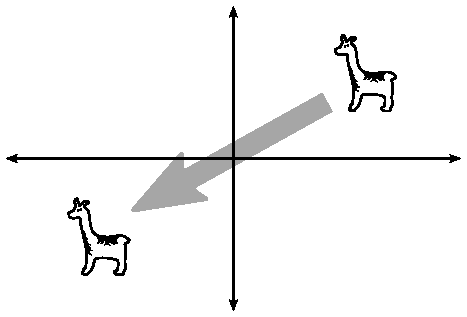
\includegraphics{transIdeaEg.pdf}
\end{image}

Pretty simple eh? We can give a more ``mathematical'' definition of a
translation involving our newly-found knowledge of matrices! Check it:

\begin{definition}
A \dfn{translation}, denoted by $\mat{T}_{(u,v)}$, is a function
that moves every point a given distance $u$ in the $x$-direction and a
given distance $v$ in the $y$-direction. We will use the following
matrix to represent translations:
\[
\mat{T}_{(u,v)} = 
\begin{bmatrix}
1 & 0 & u \\ 
0 & 1 & v \\
0 & 0 & 1
\end{bmatrix}
\]
\end{definition}


\begin{example} 
Consider the point $\vec{p} = (-3,2)$. Use a matrix to translate
$\vec{p}$ $5$ units right and $4$ units down.
\begin{image}
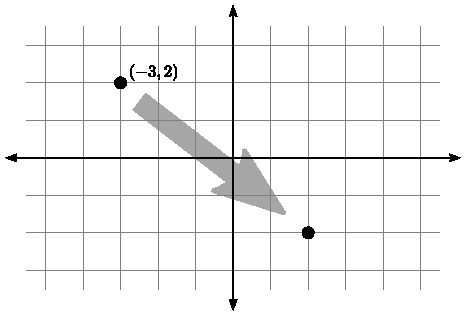
\includegraphics{transEg1.pdf}
\end{image}
\begin{explanation}
Here is how you do it:
\begin{align*}
\mat{T}_{(5,-4)} \vec{p} &= 
\begin{bmatrix}
1 & 0 & 5 \\ 
0 & 1 & -4 \\
0 & 0 & 1
\end{bmatrix}
\begin{bmatrix}
-3 \\
2 \\
1
\end{bmatrix}\\
&=
\begin{bmatrix}
\answer[given]{-3} + 0 + 5\\
0 + \answer[given]{2} - 4 \\
0 + 0 + 1
\end{bmatrix}\\
&=
\begin{bmatrix}
\answer[given]{2}\\
\answer[given]{-2} \\
\answer[given]{1}
\end{bmatrix}
\end{align*}
Hence, we end up with the point
$(\answer[given]{2},\answer[given]{-2})$. But you knew that already,
didn't you?
\end{explanation}
\end{example}

\begin{question} 
  Can you demonstrate with algebra why translations are isometries?


  \begin{prompt}
    To start we need two points, say $\vec{a} = (a,b)$ and $\vec{p} =
    (p,q)$. Now compute the distance between these two points using
    the distance formula:
    \[
    d(\vec{a},\vec{p}) = \answer{\sqrt{(a-p)^2 + (b-q)^2}}
    \]
    Now we will translate these two points using $\mat{T}_{(u,v)}$ and
    show that the distance between the translated points is the same
    distance found above. Write with me:
    \[
    \mat{T}_{(u,v)} \vec{a} =
    \begin{bmatrix}
      \answer{a + u}\\
      \answer{b + v}
    \end{bmatrix}
    \]
    and
    \[
    \mat{T}_{(u,v)} \vec{p} =
    \begin{bmatrix}
      \answer{p + u}\\
      \answer{q + v}
    \end{bmatrix}
    \]
    Now, compute the distance between $\mat{T}_{(u,v)} \vec{a}$ and
    $\mat{T}_{(u,v)} \vec{p}$:
    \[
    d(\mat{T}_{(u,v)} \vec{a}, \mat{T}_{(u,v)} \vec{p}) =
    \answer{\sqrt{(a-p)^2 + (b-q)^2}}.
    \]
    Since the distances found \wordChoice{\choice{are
        different}\choice[correct]{are the same}}, we see that
    translations are isometries.
  \end{prompt}
\end{question}



\begin{question} 
We know how to translate individual points. How do we move entire
figures and other funky shapes?
\begin{prompt}
\begin{multipleChoice}
  \choice[correct]{I've thought about this.}
  \choice{I've not thought about this.}
\end{multipleChoice}
\begin{idea}
  Well, one way to do it is to apply a translation to every single
  point in the picture. This is hard for a human to do, and usually
  requires a computer.

  On the other hand, if you can somehow group all the pieces together,
  you just move one point, and then place all the other points
  relative to the first.
\end{idea}
\end{prompt}
\end{question}


\end{document}
